\section*{3.6 正交补}
\addcontentsline{toc}{section}{3.6 正交补}
\label{sec:3.6}

在定义了正交性之后，我们现在考察相互正交的向量空间。这将在第 10 章从几何视角讨论线性降维时发挥重要作用。

考虑一个 $ D $ 维向量空间 $ V $ 及其一个 $ M $ 维子空间 $ U \subseteq V $。那么它的 \emph{正交补（orthogonal complement）} $ U^\perp $ 是 $ V $ 的一个 $ (D - M) $ 维子空间，并且包含 $ V $ 中与 $ U $ 中每一个向量都正交的所有向量。此外，$ U \cap U^\perp = \{\boldsymbol{0}\} $，使得任意向量 $ \boldsymbol{x} \in V $ 都可以唯一分解为：

\begin{equation}
\boldsymbol{x} = \sum_{m=1}^M \lambda_m \boldsymbol{b}_m + \sum_{j=1}^{D-M} \psi_j \boldsymbol{b}_j^\perp, \quad \lambda_m, \psi_j \in \mathbb{R}
\tag{3.36}\label{eq:3-36}
\end{equation}

其中 $ (\boldsymbol{b}_1, \ldots, \boldsymbol{b}_M) $ 是 $ U $ 的一组基，而 $ (\boldsymbol{b}_1^\perp, \ldots, \boldsymbol{b}_{D-M}^\perp) $ 是 $ U^\perp $ 的一组基。

因此，正交补也可以用来描述三维向量空间中的平面 $ U $（二维子空间）。更具体地，满足 $ \|\boldsymbol{w}\| = 1 $ 且与平面 $ U $ 正交的向量 $ \boldsymbol{w} $ 是 $ U^\perp $ 的基向量。图~\ref{fig:3-7} 说明了这种设定。所有与 $ \boldsymbol{w} $ 正交的向量（根据构造）必然落在平面 $ U $ 内。向量 $ \boldsymbol{w} $ 称为 $ U $ 的 \emph{法向量（normal vector）} 。


\begin{figure}[H]
\centering
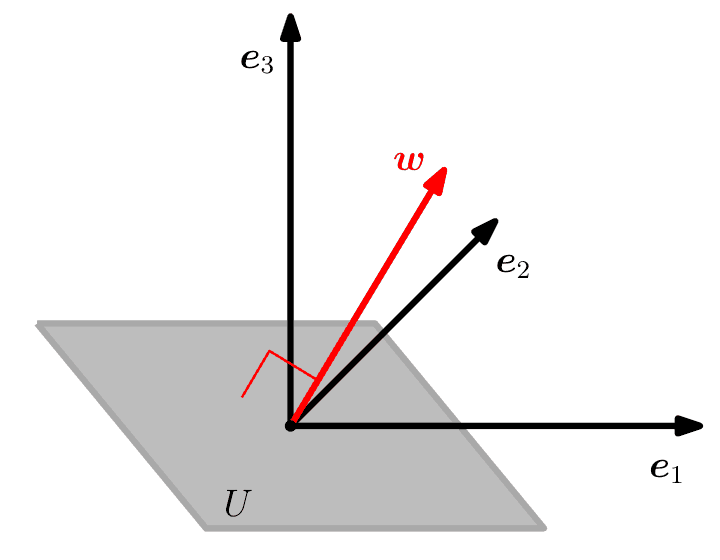
\includegraphics[width=0.92\textwidth,keepaspectratio]{docs/images/Figure3.7.png}
\caption*{\refstepcounter{figcounter}\label{fig:3-7}图~\thefigcounter 三维向量空间中的平面 U 可以通过其法向量来描述，该法向量张成了其正交补空间 U⊥。}
\end{figure}


通常，正交补可以用来描述 $ n $ 维向量空间与仿射空间中的超平面。
